\documentclass{standalone}
\usepackage{tikz}
\usepackage{pgfplots}
\pgfplotsset{width=32cm,height=18cm,compat=1.3}
\pgfplotsset{every tick label/.append style={font=\Huge}}
\usepackage{filecontents}

\usetikzlibrary{patterns}

\definecolor{citrine}{rgb}{0.89, 0.82, 0.04}

\begin{document}
	\centering
		\vspace{1.5em}
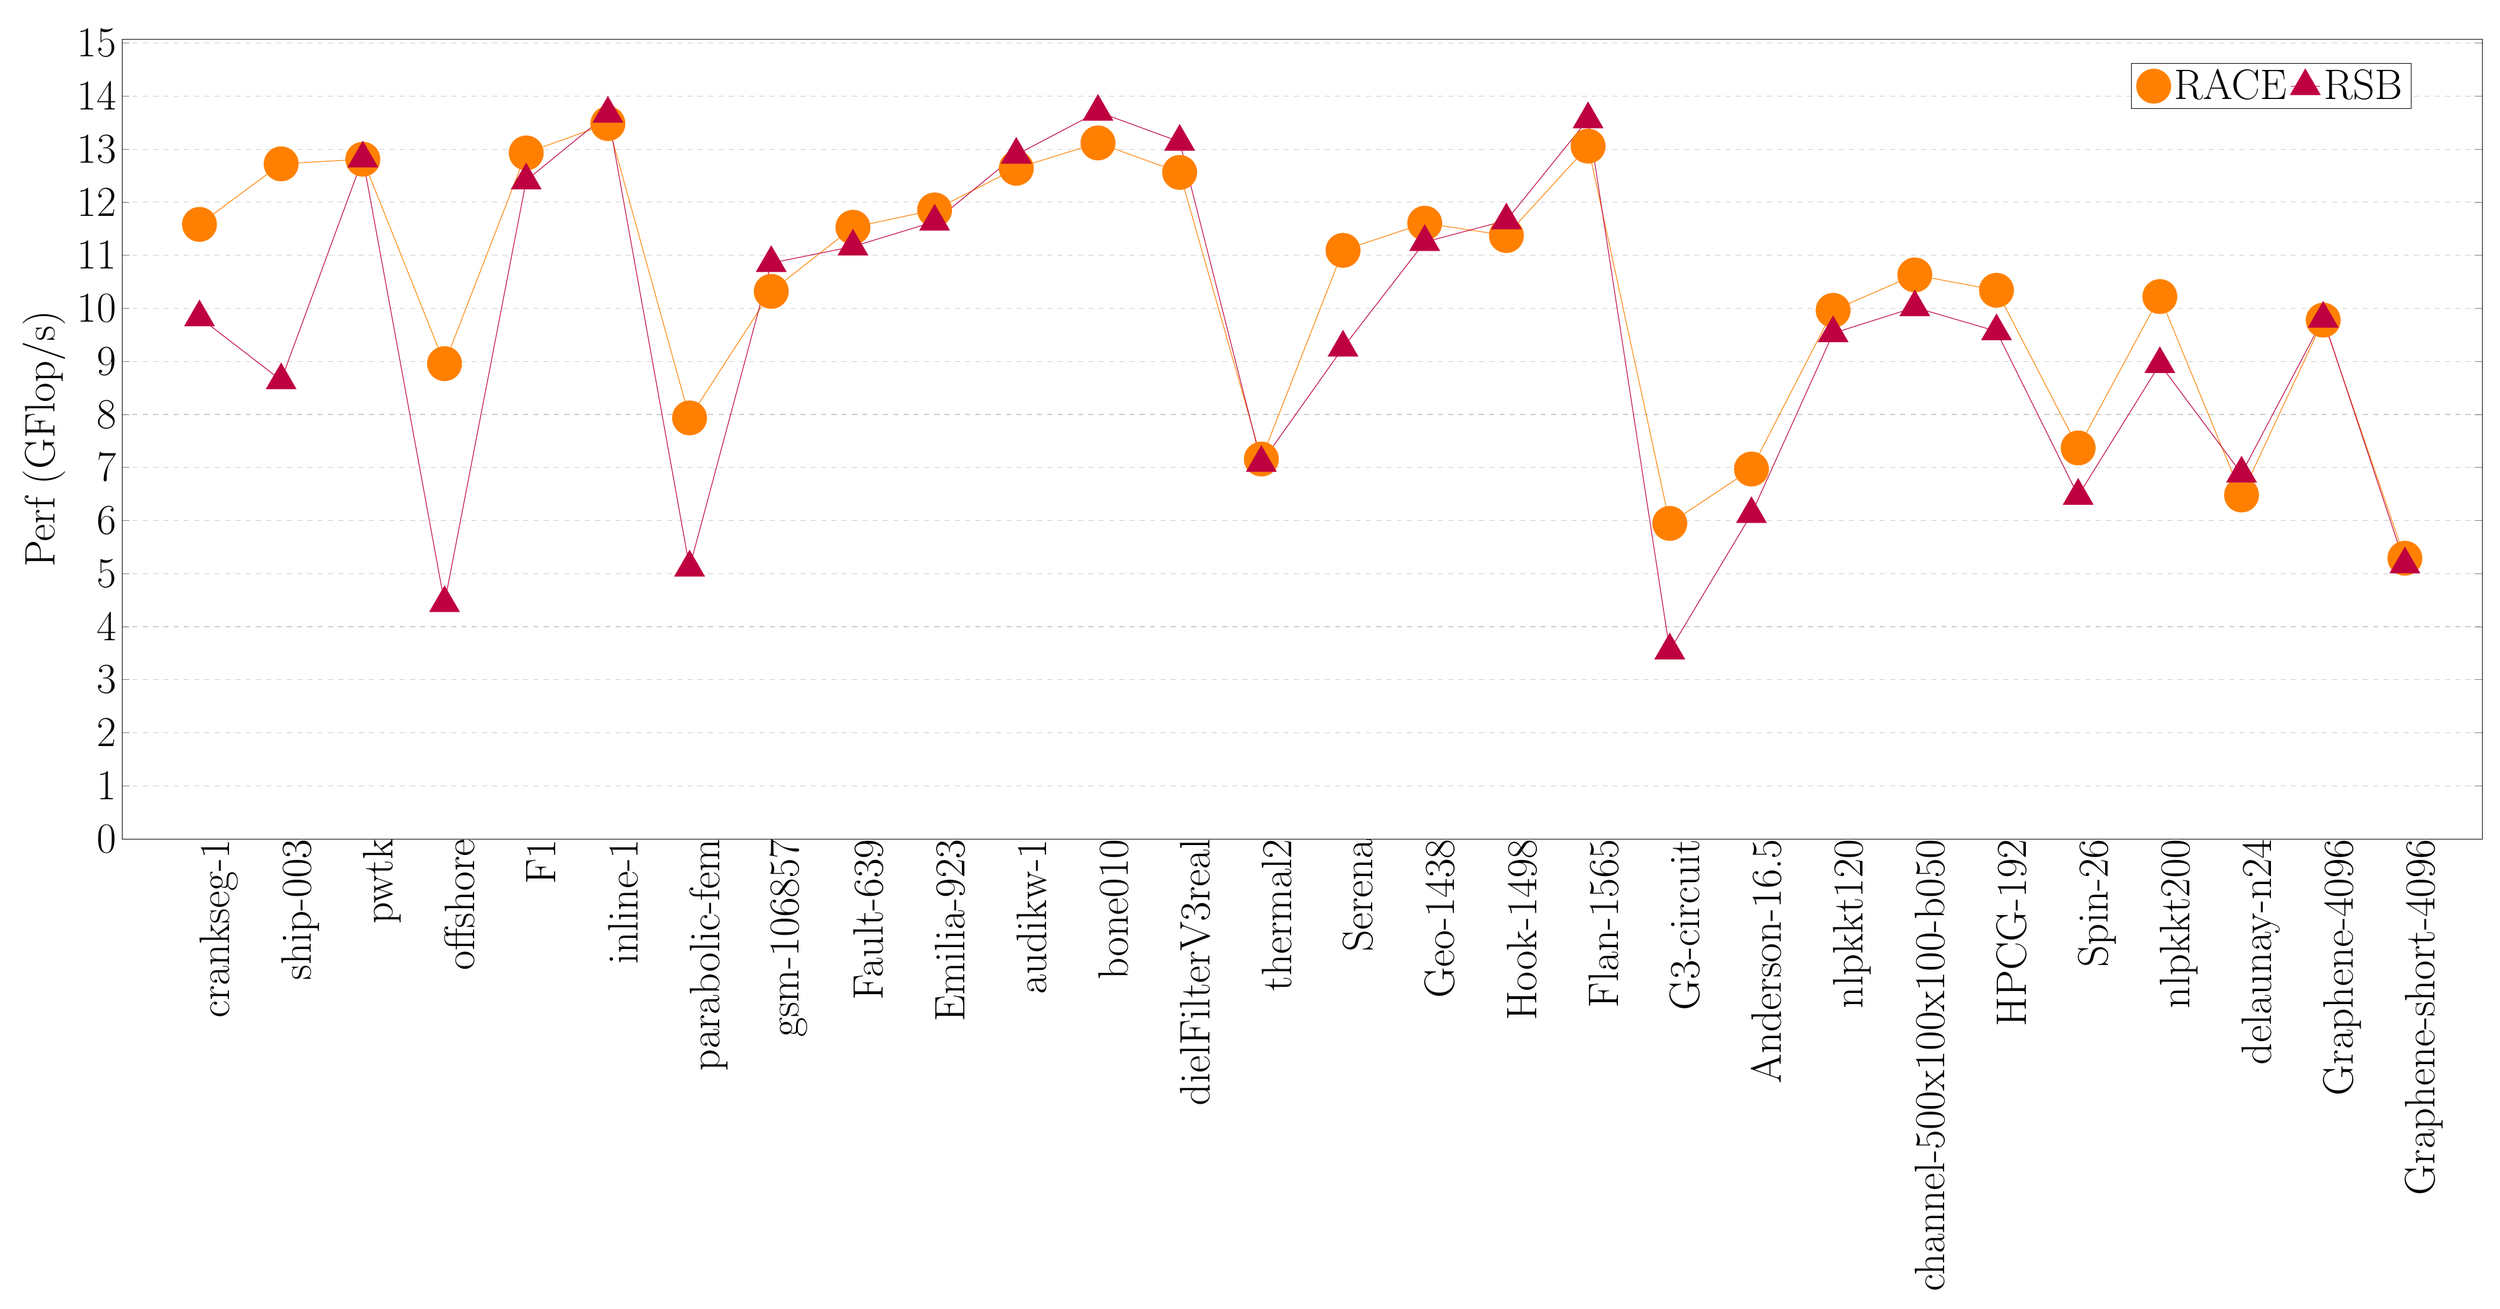
\begin{tikzpicture}
		%	\node at (13.25,15) {\LARGE{}};
			\begin{axis}[
		%	xmin=0.25, xmax=7.25,
			ymin=0, %ymax=3.25,
			xtick={1, 2, 3, 4, 5, 6, 7, 8, 9, 10, 11, 12, 13, 14, 15, 16, 17, 18, 19, 20, 21, 22, 23, 24, 25, 26, 27, 28},
		%	ytick={0,0.5,1,1.5,2,2.5,3},
			xticklabels={crankseg-1, ship-003, pwtk, offshore, F1, inline-1, parabolic-fem, gsm-106857, Fault-639, Emilia-923, audikw-1, bone010, dielFilterV3real, thermal2, Serena, Geo-1438, Hook-1498, Flan-1565, G3-circuit, Anderson-16.5, nlpkkt120, channel-500x100x100-b050, HPCG-192, Spin-26, nlpkkt200, delaunay-n24, Graphene-4096, Graphene-short-4096},
			width  = 50cm,
			height = 18cm,
			major x tick style = transparent,
			%	minor ytick={1, 5, 10, 15, 20, 25, 30 ,35,40},
			grid = minor,	
			%add_bar_commands
			ymajorgrids = true,
			grid style={dashed, gray!40},
			ylabel = {\Huge{Perf (GFlop/s)}},
		%	symbolic x coords={Graphene-2048-2048, Graphene-4096-4096, Spin-24-24-24},
			x tick label style={rotate=90, anchor=north east, inner sep=0mm, font={\Huge}},
			tick label style={font={\Huge}},
			scaled y ticks = false,
			enlarge x limits=0.035,
			legend cell align=left,
			legend style={font=\Huge},
			legend columns=-1,
			legend style={
				%at={(1,1.05)},
				%anchor=south east,
				%column sep=1ex,
				legend pos=north east
			},
			%spl_legend_code
			title= {\Huge\scalebox{1.5}{{}}}
			]

\addplot[ mark=*, mark size=10pt, mark options={orange}, draw=orange ] plot coordinates{(1,11.581950) (2,12.722942) (3,12.810374) (4,8.957090) (5,12.928522) (6,13.482575) (7,7.934556) (8,10.319803) (9,11.528034) (10,11.854632) (11,12.640306) (12,13.117369) (13,12.562132) (14,7.158996) (15,11.093061) (16,11.605302) (17,11.371847) (18,13.056664) (19,5.945987) (20,6.970780) (21,9.962605) (22,10.629349) (23,10.340284) (24,7.368607) (25,10.221975) (26,6.481632) (27,9.777899) (28,5.289580)};
\addplot[ mark=triangle*, mark size=10pt, mark options={purple}, draw=purple ] plot coordinates{(1,9.829810) (2,8.642974) (3,12.824990) (4,4.443132) (5,12.410470) (6,13.667295) (7,5.114396) (8,10.853765) (9,11.164475) (10,11.633707) (11,12.895039) (12,13.703456) (13,13.139291) (14,7.086881) (15,9.258430) (16,11.249399) (17,11.656714) (18,13.562491) (19,3.552169) (20,6.122011) (21,9.530124) (22,10.018854) (23,9.567151) (24,6.466166) (25,8.949014) (26,6.885692) (27,9.804079) (28,5.174290)};
	%addplot cmd

	\legend{RACE, RSB}

	\end{axis}			
\end{tikzpicture}

\end{document}

